\chapter{Discussion and Conclusion}
% (was sind die broaden takeaways von meinem Kram)
% * Nochmal nen theoretisches Embedding, Kontextualisieren für Bildungsressourcen
% * ...and conclusion

The results generated thus far should finally answer our research questions and check if the general thesis goals were achieved. In this section, we will first interpret the generated results iteratively to be able to assess the performance of the algorithm on the dataset. On the basis of that, an answer to the general question if the methodology is applicable for the domain will be formulated. This is followed by a discussion of the algorithm in itself from the perspective of somebody that worked with it extensively. Finally the architechture is quickly discussed and the thesis concluded.

\section{Interpretation and Discussion of results}
%Research Question: Ich will die Methodik von dem Paper auf educational resources Applien. Das unbedingt in discussion & conclusion aufgreifen.

First we evaluate our implementation by comparing its performance for the placetypes-dataset and discussing possible reasons for any discrepancies. Following that, we will discuss the results for the Siddata-dataset when compared to those of the literature to see if the algorithm can cope with the domain transfer. On the basis of which we will try to find an answer to the question if the general methodology is able to cope with the domain in question. Afterwards we will discuss the results of the hyperparameter-search and its implications on our dataset.

\subsection{Results for Placetypes}

When doing classification with decision-trees it is a design-decision to either train one decision-tree per class that just classifies if a sample is that of that class or not (\textit{1vsRest}), or alternatively generate a single tree that must predict the exact class membership for all classes at once (\textit{AllAtOnce}). In \autoref{tab:f1_geonames_foursquare_all}, we reported the results for both of these conditions. 

The results indicate that performances for depth-limited trees are not consistently worse than unbounded trees. This is not suprising, considering that decision trees are known to be prone to overfitting, which can only really happen for unbounded trees. Similar results were reported in the work of \textcite{Ager2018}.

The best results were achieved for the condiditions \textit{balanced 1vsRest} and \textit{unbalanced AllAtOnce}. In general the results indicate that especially for depth-limited trees it holds that for single \textit{AllAtOnce} classifiers, balancing is bad for performance an vice versa. Considering that depth-limited ones can only predict very few classes explains why the \textit{AllAtOnce} condition performs badly overall. For the same reason, however, these classifier benefit from unbalanced datasets - without balanced sample-weighting, these trees can just detect the most common class labels and assign them, which was shown to be the case here as well. Generally however, especially for depth-limited trees, \textit{1vsRest} improves performance.


\subsubsection*{Explanations for good results}


As shown in \autoref{tab:f1_mainalgos_me_short}, the achieved results outperform those of the literature for the placetypes-dataset in all cases, often with a significant margin. Considering that this implementation replicates \cite{Derrac2015} without major algorithmic improvements and does not contain some of the improvements of \cite{Ager2018, Alshaikh2020}, this is initially surprising, so here we will discuss some possible explanations for that.

\paragraph{Errors} 
Naturally, the first thing to to in this situation is to check for errors in the implementation. In following that route, however, it is important to keep in mind that errors in the actual algorithm are an unlikely candidate for an erroneously high performance. As elaborated before, the performance of the decision-tree is only a surrogate metric to evaluate the resulting semantic directions. Among others this implies that the classification target for the task is disregarded in all algorithm steps except the final evaluation with the decision trees. As long as that is given,  the only realistic source of error that leads to higher-than-expected accuracies reliably is thus in this step. This does not mean that there are certainly no errors in the implementation of the rest, but as long as the classification target is not used, all these errors would only coincidentally lead to better classification results. In contrast to that, there are many sources of errors in the decision tree classification that will likely lead to unrealistically high performances such as mixing up the training- and testing set. In any case, both the algorithm itself and the decision-tree classification was triple-checked for errors and many sanity-checks were performed that all lead to the same conclusion, so from now on we will assume that the results are correct and discuss possible reasons for that\footnote{The code is open-source and available at \url{github.com/cstenkamp/derive_conceptualspaces}, and \me is thankful for any issues.}


\paragraph{One-Vs-Rest-Classification}

\cite{Ager2018, Alshaikh2020} are both unclear if they did the former or the latter. Generally, All-At-Once would be the harder task and comparing accuracies of 1vsRest to AllAtOnce an unfair comparison. However, there are a few things that can be assumed:

Both of them report to have used the sklearn-implementation of decision-trees, just like this work. This specific implementation reportedly uses the CART algorithm \cite{breiman1984classification}, which only allows binary trees, where every node has exactly two children\footnote{\url{https://scikit-learn.org/stable/modules/tree.html\#tree-algorithms-id3-c4-5-c5-0-and-cart}}. Consequently, a decision tree of depth one can only classify $2^1 = 2$ classes, whereas a tree of depth two can classify up to $2^2=4$ classes. 
%TODO: actually for depth 2 it's 2^2 + 2^1 + 2^0 = 7 and thus for depth 1 = 3 
Due to that, the best achievable accuracy of a perfect depth-1-tree is $\frac{\text{||samples in two most common classes||}}{\text{||samples in all classes||}}$, which is $\frac{176+74}{403} = 0.62$ in the case of GeoNames and $\frac{88+82}{391} = 0.43$ for Foursquare.\footnote{Note that these values only hold on average, as the samples are arbitrarily assigned to the train- and test-set.} The latter value is lower than what \cite{Alshaikh2020} report, indicating that is not how the authors generated results. This would be even a lot more pronounced when classifying the movie genre, which has 100 classes. 

Also semantically it is reasonable to assume to do 1vsRest: they state extensively that they are looking for a direction for \textit{scarieness} in movies, where the genre corresponding to that \textit{(Horror)} is only one of the genres. This kind of mapping Genre-FeatureDirectionPredictingGenre can only be found with separate trees per genre - and thus generally per class. Both of these reasons lead us to the assumption that they likely also did a separate tree for each of the features.

\paragraph{Dataset size}
Only a small subset of samples even \textit{have} a class assignment (403 of 1383 in 7 classes in the case of GeoNames (see \autoref{fig:scatter_mds_placetypes}), 391 in 9 classes for Foursquare), and the classes are heavily imbalanced (GeoNames between 176 and 14 samples per class, Foursquare between 88 and 6). We used the classes as uploaded by \cite{Derrac2015}\footnote{\url{https://www.cs.cf.ac.uk/semanticspaces/}}, of course there is the chance that they did not make all of their data publicly available, whereas \cite{Ager2018, Alshaikh2020} had access. Furthermore, that is generally a tiny dataset so the statistical power of any result here is really low - maybe it is just coincidendence

\paragraph{Not having some improvements of \cite{Ager2018}}
The contributions from \cite{Ager2018} were primarily the Fine-Tuning and the condition where averaged word-embeddings are used instead of \gls{mds} (denoted \textbf{AWV}). As can be seen in \autoref{tab:f1_placetypes_long}, these contributions do not seem to affect the classification performance much, being in the same region as those for their MDS-condition which is implemented here as well: There are no really significant improvements that are not given here, giving no reasong to assume that their performance should be superior.  

\paragraph{Not having some improvements of \cite{Alshaikh2020}}

The \textbf{Ortho} condition of \cite{Alshaikh2020} actually does significantly outperform the base algorithm for many configurations. For Foursquare, their performance comes very close to mine, whereas their GeoNames-performances are a lot worse than mine. Apart from that, if the code uploaded by \cite{Alshaikh2020} is really the basis for their implementation, ther are strong reasons to doubt what they claim to do and what they actually do really matches. A quick inspection of their uploaded source code\footnote{\url{https://github.com/rana-alshaikh/Hierarchical_Linear_Disentanglement/blob/master/Hierarchical_Linear_D4.py\#L485-L486}} revelaed for example they take the kappa-score from on the raw predictions, not on the rank like \cite{Derrac2015} described and like we do (see \autoref{tab:kappa_measures}) and also do not apper to weight the kappa-scores. Apart from observations like this, it is hard to say more about their code, because the two files uploaded by them are not the whole algorithm and also depend on loading many files that are not in the repository, and also none of the evaluation on basis of decision tree performance is in the repository.

\paragraph{Using the best configuration}

Another difference appears to be that we looked for the best configuration \textit{for this particular task}, which is a different one for each combination of dataset $\times$ \gls{dt}-depth $\times$ classification-target. It appears from their description that \mainalgos did hyperparameter-tuning before, using another possibly subjective metric, and then decided on one (or rather four, see \autoref{tab:f1_placetypes_long}) configuration that was not optimized for the dataset $\times$ \gls{dt}-depth $\times$ classification-target. It should be noted that in this work, the algorithm is also not optimized for that task, but only the best of the 80 different parameter-combinations that were executed is used respectively. At the same time however, some way to find a hyperparameter-configuration has to be used, and it is unlikely that \mainalgos chose the worst configuration. \autoref{tab:f1_geonames_foursquare_all} displays robust results of a parameter-configuration that proved good on average. As these results, however, also outperform those of \mainalgos significantly, choosing the best configuration seems to play only a minor role for the performance.

\paragraph{Weighted Average of the individual classifiers}

The considered scores for the 1vsRest-condition of this work are calculated from the scores of the individual per-class classifiers both with uniform weighting per class (bottom two rows of \autoref{tab:f1_geonames_foursquare_all}) and also with class weights inversely proportional to class size (middle two rows). Clearly, the condition that weights the indiviudal scores leads to better results. Weighting the score is a reasonable assumption, given that the individual class frequencies are very imbalanced (see \autoref{fig:scatter_mds_placetypes}). Unfortunately, \mainalgos do not explicitly share if they calculated weighted class scores as well. If we assume for now that \mainalgos did report unweighted scores and thus disregard the condition where class-scores are weighted (see bold scores in \autoref{tab:f1_geonames_foursquare_all} or last column of \autoref{tab:f1_placetypes_long})), our results are still comparable with those of \mainalgos and especially in the case of GeoNames-labels a lot closer to those reported in the literature. So while we hereby argue that weighting the scores makes sense, even if that is not the case our results are still acceptable. Again it should be stressed that there are only really few and imbalanced labels for this dataset in general, making the statistical power of these results very small.

\paragraph{Improvements that we do have}

We do not have many differences in hyperparameters or algorithm-components than \mainalgos do, but there some. For example using tf-idf as \gls{quant} instead of PPMI: Close inspection of \autoref{tab:best_params} shows that often, the tf-idf results are superior to the PPMI-results, and sometimes the combination of using tf-idf as quantification and tf-idf as dtm-quantification is good. This may lead to two conclusions: Either tf-idf is just better than PPMI under certain conditions, or just that the fact that more different results generated here just increased the statistical chance that good results were among the generated ones.

\subsubsection*{Conclusion} 

Even though this work did not do much beyond \mainalgos, maybe there were some small things that were done here that gave an edge, such as trying out different or just more hyperparameter-combinations. Maybe the scores here were calculated differently than in \mainalgos, but even if that were the case the results generated here are still comparable. Maybe our implementaion had errors, maybe those of \mainalgos had, but in any case as the dataset is so small exact results do not seem incredibly informative anyway. Most importantly the comparison was performed to check if this implementation is working correctly, and the evidence for that appears very strong.

\subsection{Results for educational resources}

One of our two research questions was to figure out if the methodology works for our domain. So now that we have established that the implementation seems to work on other datasets, we finally look how the algorithm copes with the Siddata-dataset.

\subsubsection{Quantifiable dataset differences}
\label{sec:discuss_datasetdiffs}

When describing the datasets in \autoref{sec:datasets}, we noticed that they are quite different. An important difference from our to the originally used datasets is, that in our dataset the relationship between how relevant a concept is for an entity and how often its words occur in the respective \gls{bow} is not given. Furthermore, the Siddata-dataset contains far less words per entity: the median number of unique words per description is three orders of magnitude smaller compared to the placetypes-dataset (see \autoref{tab:summed_unique_words}). Even though the number of entities in the dataset is higher, in sum it contains substantially less unique words. The difference is very prominent in relation to the dataset size (indicated by the last two columns). Because of this, for most of the \glspl{ngram} that serve as candidate-terms in the subsequent classification the positive class (\textit{entities that contain the phrase}) is far smaller than the negative class. 
% As established, a very important difference is that more relevant words do not occur more often. We assumed  because of that, the kappas that compare rankings are not so good

\textcite{Derrac2015} extracted roughly 20\,000 candidates for the movies- and placetypes-datasets. If the same number of candidates were to be extracted in our case, more than half of them would occur in less than 25 descriptions, such that the positive class for the corresponding classification problem contains only $\frac{24}{26346} \approx 0.09\%$ of the samples. It seems unlikely that even class weighting can make up for that, yielding a bad classification. Because of this, it is justified to consider less entities. To improve the ratio of classes, it was accordingly decided to only consider entities of at least 80 words (see \autoref{tab:corpussizes}), which yielded the final number of 11\,601 considered entities. 

When discussing the dataset differences in \autoref{sec:results_datasetdiffs}, we assumed that the dataset differences will likely lead to less candidates being extracted. This is confirmed by the results: \autoref{fig:candidate_histogram} shows that the number of candidates that apply to each entity is exponentially decreasing. The score represents a low \textit{faithfulness} in the representational capacity for many of the produced candidates. This indicates that there is a much variability in the dataset that is not explained by any of the extracted words. A consequence of this is that mapping this space onto a limited number of extracted directions will lead to a loss of information which does not model the full latent information.

% The #Texts containing a candidate are exponentially decreasing, which means that for many of the candidates that ARE produced the classification to measure the faithfulness has a really hard time

Despite the small number of extracted candidates however, a sample run with 200 dimensions still yielded 5016 phrases with $\kappa \geq 0.1$ ($T^{0.1}$) and 1008 with $\kappa \geq 0.5$ ($T^{0.5}$), which is enough for the algorithm, considering that for a 200-dimensional embedding only 400 values with $\kappa \geq 0.5$ would be necessary. However, there are far less ones in $T^{0.1}$ compared to \textcite{Derrac2015}, meaning the resulting clusters are considerably smaller. 

This, however, is not necessarily a sign of bad performance of the algorithm: The number of cluster-elements that \cite{Derrac2015} for the 200-dimensional \gls{cs} for the placetypes dataset (see \autoref{tab:generated_stats}) is 21\,819. Considering that they considered  number of candidate is 21\,833, the threshold does not meaningfully reduce the number of considered words. Accordingly, in this dataset all extracted words (which are all words with $\gls{df} \geq 50$) are considered in the final embedding. This leads to high amounts of noise, \ie a bad modelling of the actual latent topics. 

Increasing the threshold a candidate to be considered a \textit{faithful} representation also does not help: Consider the \textbf{Sum} column of \autoref{tab:generated_stats}. The first two rows of \autoref{tab:generated_stats} display sample results of \gencite{Derrac2015} original implementation for the domains of movies and placetypes as it was uploaded by the authors. Let us consider the Sum column, which indicates how many unique terms have been identified and used as \textit{most important feature direction} among all different uploaded conditions. The authors uploaded their results for embeddings of the dimensionality 200, 100, 50 and 20, in each of which the number of extracted cluster centers  was 2*ndim. Considering this, the minimal number of cluster centers that could be extracted among all their uploaded results is 400. The worst case would be given, if the sets of \textit{salient} terms for each of these runs would be completely mutually exclusive. In that case, not a single term that was considered \textit{salient} by one of these results would considered salient by any other configuration, such that the sum of unique terms extracted among all combinations is 400+200+100+40=740. This can be seen as a measure of \textit{Robustness} of the algorithm. If different parameter-combinations or just different initial random number generator results have a high impact on the generated results, the algorithm is not robust. In the case of our algorithm this shows in different extracted candidate terms. For the placetypes-dataset, 697 different semantic directions are found. Considering the condition $\kappa \geq 0.1$, 21\,832 of the 21\,833 candidates were considered salient among the runs. This indicates much noise in the dataset that obfuscates the latent information.

These observations lead us to the conclusion, that extracting less candidates may better capture the semantic content of the dataset. The disadvantage is that the resulting embedding captures less variance of the original dataset, however, those directions that are extracted show increased robustness. This is also indicated by the lower number of uniquely extracted candidates summed over all run-configurations in \autoref{tab:generated_stats}. 

When discussing the dataset, we already theorized that only keeping those entites for which a classifier can successfully predict its faculty may help to increase dataset quality. That turned out to be not necessary but would still be a good future research opportunity. Another possibility that could have been considered in the case of low performances is to use only the 1500 with the longest descriptions, bringing its distribution closer to the placetypes-dataset (but still not changing the properties). 

% \todoparagraph{or only those ones where BERT can sucessfully }classify the faculty. Again, faculty is not everything, BUT if the faculty CAN be extracted, cases that only list names or places are out (...except FROM the name of place follows the faculty but lets ignore that)

In sum, our previous hypothesis that the different dataset statistics leads to different conditions for the algorithm seems confirmed by the intermediate results. On the other hand, the final classification performances (\autoref{tab:robustresults_perfb}) are proof some important information of the dataset is captured regardless. In fact, not only are enough candiates extracted by the algorithm, but the results even indicate less sensibility for different hyperparameters for our dataset compared to the results of \cite{Derrac2015} for the placetypes-dataset. Regarding the algorithm, our results indicate that the methodology is robust and does not only work for datasets with the aforementioned properties.

\subsubsection{Classification results}


% The plots \ref{fig:scatter_mds_movies} and \ref{fig:scatter_mds_placetypes} show a 2D-representation of the MDS %TODO: link MDS anyway, if not to the glossary than to the section
% of the movies- and placetypes-dataset as made public by \textcite{Derrac2015}.\footnote{\url{https://www.cs.cf.ac.uk/semanticspaces/}} Visually comparing them to their equivalent to the Siddata-dataset (\autoref{fig:scatter_mds_siddata}) 
% \todoparagraph{shows that while the movie-embeddings looks pretty clustered}, the clustering of the placetypes-dataset looks in fact a lot worse than that of the Siddata-dataset.
% %TODO: obviously write again. What do we see? A 2D-Version of the MDS. If we see very distinct clusters in that, we can conclude that it sounds possible that we can detect whatever-we-colored-by from this embeddings to an okay degree.

Comparing the \gls{tsne}-embeddings of the classification problem associated with the Siddata-dataset (\autoref{fig:scatter_mds_siddata}) with the one of the placetypes-dataset (\autoref{fig:scatter_mds_placetypes}) indicates that the former seems to be more prominent in the data. This saliency of the faculty in the representation of the samples is further confirmed by the fact that both our implementation of BERT and even representation relying on only three dimensions achieve reasonable performances on the data.

We should keep in mind that the problem appears to be comparably easy when evaluating our performance. Despite this, our acccuracies are suprisingly good: Our algorithm robustly achieved  81.4\% accuracy with depth one trees, which is comparable to the accuracy for BERT (85.19\%), and by far outperforms the 3D-embedding (64.3\% weighted accuracy). This indicates that our method indeed finds terms that accurately predict the faculty among its salient directions. A classifier that that uses only three dimensions is already better than BERT, and the unbounded one has 94.3\% classification accuracy. This stands in contrast to the results of \cite{Ager2018}, who report that their depth-1 trees achieved the best overall performance. In contrast to the placetypes-dataset, unbound trees for this dataset appear not to be overfitting. This can be explained by less noise and general variance in our dataset. Another interesting observation from these results is that the variance is on average comparably low, indicating robustness. 

Unbounded \glspl{dt} are actually only an answer of the question if it can recover at least one property from the dimensions, not how important one or any of the dimensions are. So their good performance is only a measure of the question if the information about the faculty is not lost through the embedding.

Interestingly, classifying all faculties at once performed a lot worse in case of the Siddata-dataset (\autoref{tab:robustresults_allatonce}). This difference in performance is a lot more prominent than it was for the placetypes-dataset. % \todoparagraph{AND WHY COULD THAT BE?!}. 
Considering this, a fairer comparison to BERT would have be to also split the dataset into several \textit{1vsRest} problems.


When looking at the individual faculties, we see that for the faculty \textit{Humanwissenschaften}, depth-1-trees perform a lot worse than for the other faculties, but also shows a large standard deviation (\autoref{fig:faculty_boxplots} shows this even better). This indicates that the classification performance for this faculty strongly depends on what ends up in the train set, leaving the interpretation that the individual descriptions of courses belonging to this faculty have a higher degree of variance in their descriptions. This is an interesting result, as we would have expected other faculties that contain many different courses of study to have a higher variance. % Considering that this one is even one of the larger faculties of the dataset 

% This is a bit surprising: We would have rather expected Erziehungs-/Kulturwissenschaften is more diverse with Lehramt in it.  Interestingly, preliminary analysis of Johannes and SidBERT (unpublished) showed that Mathe/Informatik (top-1 25.7\%, top-5 42.1\%) and Sozialwissenschaften (top-1 32.7\%, top-5 65.5\%) are most problematic (in the sense that their neirest neighbor embedding is not from the same faculty), followed then by Humanwissenschaften. Also the class frequency for that class is not the culprit, its one of the larger ones.

While these quantitative results look very good, it is important to stress that they only refer to how good the faculty can be detected from the semantic directions, which is only one (apparently very prominent) property of the data. Evaluating the algorithm this way is in line with the literature \mainalgos, but does not test everything the algorithm does or how it may perform with respect to other human concepts among the data. In our evaluation, we also evaluated the algorithm on its performance when classifying the first level of the \gls{ddc} as detected by SidBERT with similar performances.\footnote{\url{https://github.com/cstenkamp/derive_conceptualspaces/blob/main/notebooks/analyse_results/siddata/decisiontrees_bestconfig.ipynb}}. As, however, the categorization system of that shows high similarity to the categories made up by the faculties, the results for these are not printed in this work. Other avenues may include to try to detect the \textit{difficulty} of a course on basis of average grades, the \textit{interdisciplinarieness} on basis of the number of students from other faculties attending it, or the \textit{effort} required for it with labels generated from the amount of ECTS a course provides. Unfortunately, metrics are not present in the current dataset. Ultimately, the best way to objectively quantify the quality of the directions remains to perform studies with human subjects evaluating their subjective appeal.

\subsubsection{Dataset Quality}

Now that we have established that we have reason to assume that our algorithm is good, let us interpret some results with respect to the dataset. We have extensively discussed our dataset with respect to the frequencies of words, let us now try to see if we can speculate about some more of its properties.

Among others, we are interested if any important information gets lost when using only the extracted semantic directions to embed the entities. The results for unbounded decision trees (\autoref{tab:robustresults_perfb}) which achieve 94.3\% weighted accuracies indicate that at least regarding information about the faculty seems to not get lost. This indicates again that our directions are useful to express the variance in the data, considering that the results for the faculty are not trained on but are only a side effect of the extracted semantic directions. 

Another method conducted to test how much variance in the dataset is explained by the semantic directions was to check how many dimensions and what amount of discretisaton was required such that multiple entities fall onto the same position in the left-over vector space. \autoref{tab:duplicates_per_comb} shows how many dimensions are required such that enough entities are unambiguously defined. The results indicate that without much discretisation of the space, a small number of directions is enough such that no duplicate positions will be taken. This indicates that much of the variability in the original data can be explained by a small number of dimensions. Considering however that these are random directions, it also indicates a high correlation/linear dependency of the dimensions that are left over, otherwise this would only hold if the leftover directions happen to be the good ones.

It is, however, much more interesting to analyse which of the entities did become duplicates through this. \autoref{tab:same_embed} shows a sample where three out of four entities that landed on the same position refer to the same course of different years. Results like this indicate that all results concerning ambiguity of samples must be taken with a grain of salt, as the dataset even in its cleaned form seems to still contain many duplicates.

\begin{table}[h]
    \centering
    \resizebox{\textwidth}{!}{%
    \begin{tabular}{r|ccc}
    \textbf{Course Name} & \multicolumn{3}{c}{\textbf{Leftover Dimensions}} \\ \
    & strukturierten & internationales & 1950er \\ midrule
    !! FÄLLT AUS !! Anna Seghers: Das siebte Kreuz (1942) & 2              & 15              & 18     \\
    Anna Seghers: Das siebte Kreuz (1942)                 & 2              & 15              & 18     \\
    Anna Seghers: Das siebte Kreuz (1942) (NDL 2)         & 2              & 15              & 18     \\
    Friedrich Hebbel: Agnes Bernauer (1852)               & 2              & 15              & 18    
    \end{tabular}%
    }
    \caption{Sample courses falling onto the same embedding after discretisation}
    \label{tab:same_embed}
\end{table}

% btw diese table auch shcreiben dass "der space nicht genug ausgefüllt ist", course of dimensionality, in 3D ist like 80\% des unitcubevolumens im unitball, im 200D nur like 0.00001\%

% \subsubsection{Qualitative analysis}

% * Regarding "Dass ich immer die beste config genommen hab aber durchgehend neue generiere, weswegen viele plots inkompatibel (zeigen andere semantic directions und andere werte für accuracy undso) sind aber alle zeigen halt nice sachen":
%   * erstmal wenn ich die cosine distance von "stadtgeographie" und "tourismus"  oder "psychologie" und "gehirn" anschaue sind die extremely nah
%   * Die highlights die ich präsentier sind von verschiedenen params und blablabla
%   * One thing is important: The NAME itself is irrelevant for the classification performances!! Only the direction is relevant
%     * bei den namen ist nur die human-interpretability aus, und die tatsache dass verschiedene aber sinnvolle rauskommen ist eher ein feature als ein bug



% \paragraph*{Which ones DO miscalssify?}


% wenn man sich anschaut WAS denn falsch klassifiziert wurde sieht man halt dass die Kurse die offensichtlich nicht Mathe sind eben falsch klassifiziert wurden, oder dann eben "logic" in mathe landet, well it's not wrong, it's the dataset 

% * and also keep in mind that there are quite a few courses with shitty descriptions!
% * LETS analyse THOSE THAT MISCLASSIFY
%     * When training one with 93.53\% weighted mean acc on the full data it achives 97.85\% accuracy, that's A LOT
%     * ...it is not the case that only those with "tutoren: xyz" are misclassified, like we thought.

% Examples: see decisiontrees_bestconfig.ipynb at the bottom




\subsubsection{Qualitative analysis of the extracted dimensions}

\autoref{tab:courses_top3} shows the extracted feature directions that, according to a \gls{dt} classification, best predict a faculty. Many of the extracted features are subjectively very appealing in encoding the faculties - in some cases even extracting the exact faculty name. \autoref{fig:dims_for_fb} displays the results from another hyperparameter-combination, which are similarly convincing. In a recommendation system, many of these directions would make sense as features semantically describing a course. \autoref{tab:clusters} shows some exemplary terms that make up a cluster. These look intuitively appealing as well.

When looking at the examples per faculty, we observe mixed results. On the one hand, \eg \textit{erziehungswissenschaft} is perfeclty on point, on the other hand the extracted terms for faculties for \textit{Physik} and \textit{Biologie/Chemie} did not look convincing in a single run. One possible explanation may be low class frequency. Both mentioned faculties are among the smaller classes, but so are \textit{Mathematik/Informatik} and \textit{Wirtschaftswissenschaften}, both of which are generally classified really well.

% Would you want to take the words from the top 3 direcitons as names from the dimension? Some of them definitely: erziehungswissenschaft, programmiersprache, "deutsch literaturwissenschaft", "psychologie", "arbeitsmarkt"... but some of them meh.


% * "The results of the top 3 directions per faculty will be elaborated further in the discussion" 
% * also \autoref{tab:highest_ranking} and \autoref{fig:dims_for_fb}
%     * "erziehungswissenschaft" für Erziehugnswissenschaft
%     * "deutsch literaturwissenschaft" für Sprach/Literaturwissenschaften
%     * "stadtgeographie"/"tourismus" für kultur/Geowissenschaften
%     * "gehirn" oder "psyhcologie" für human? GOLD
%     * "juristisch" für rechtsiwssenschaften
%     * "programmiersprache" für Mathe/Info


% * Mechanik für Mathe/Info was a bad one but exception
% * Again, Physik and Bio/Chemie
% * Ich hätte halt auch die dimensionen die es predicten averagen können huuiii


\paragraph{Do bad performances correlate with bad feature names?}

% * Physik and Biologie/Chemie are bad and were so in almost all runs


In almost all results, the extracted dimensions for the faculties \textit{Physik} and \textit{Biologie/Chemie} appeared the worst. The results for these faculties show the highest variance and do not make much intuitive sense. The top extracted directions (\autoref{tab:courses_top3}) show that the dimensions are good, explaining why even the performance of depth-one-\glspl{dt} is good. Quantitatively, we observed the worst performances for the faculties \textit{Humanwissenschaften}, followed by \textit{Physik} and \textit{Biologie/Chemie}. Looking at \autoref{tab:courses_top3} shows reasonable results for all faculties except for \textit{Biologie/Chemie} and \textit{Physik}. That is interesting: Even though for \textit{Humanwissenschaften} the performance is generally not too good, the dimensions we extracted from it are plausible. % Other directions extracted for this faculty include \todo

\paragraph{Are intuitively appealing phrases among the semantic directions?}

\begingroup

\renewcommand{\arraystretch}{0.75}
\begin{table}[H]
	\begin{tabular}{rcccc}
	\toprule
	 \textbf{NDim} & \multicolumn{2}{l}{\textbf{50}} & \multicolumn{2}{l}{\textbf{200}} \\
	 & \textbf{0.1} & \textbf{0.5} & \textbf{0.1} & \textbf{0.5}  \\
	\midrule
	computer & 24 & 0 & 4 & 11 \\
	sport & 10 & 12 & 4 & 11 \\
	recht & 27 & 0 & 11 & 4 \\
	musik & 17 & 12 & 7 & 8 \\
	management & 25 & 0 & 9 & 6 \\
	literatur & 0 & 0 & 0 & 0 \\
	sprache & 22 & 0 & 9 & 6 \\
	psychologie & 23 & 2 & 3 & 12 \\
	wirtschaft & 25 & 0 & 13 & 2 \\
	geographie & 28 & 0 & 10 & 3 \\
	schule & 17 & 8 & 7 & 6 \\
	kultur & 22 & 0 & 5 & 8 \\
	wissenschaft & 17 & 0 & 14 & 0 \\
	sport & 10 & 12 & 4 & 11 \\
	N & 38 & 38 & 15 & 15 \\
	\bottomrule
\end{tabular}
\slcaption{Number of appealing phrases found among the directions. Results show the number of parameter-configurations in which the respective word was extracted as direction. Last row indicates how the how many configurations are considered for each column.}
\label{tab:appealing_phrases}
\end{table}
\endgroup
	

In \autoref{sec:pre_qual_an}, we decided on some terms that would make intuitive sense as semantic directions. The results from \autoref{tab:appealing_phrases} show that many of these were actually used as candidates robustly among many different parameter-combinations. This is a very promising result, especially considering that the actual document frequencies for these terms are comparably low, making the result even more astonishing and indicating robustness by how many different configurations found these teerms to be significant. \\

\vspace{-3ex}

\begingroup
\renewcommand{\arraystretch}{0.75}
\begin{tabular}{lll}
    computer     & 1.0\% \\
    mathematik   & 0.8\% \\
    mathe        & 0.0\% \\
    wissenschaft & 3.3\% \\
    recht        & 4.16\% \\
    musik        & 2.27\% \\
    sport        & 1.03\% 
\end{tabular}
\endgroup
\vspace{0.5ex}

Some of these phrases even regularly end up as a deciding factor to detect one of the faculties in the decision trees, such as \textit{computer} for \textit{Mathe/Informatik}, \textit{psychologie} for \textit{Humanwissenschaften}, \textit{Schule} for \textit{Erziehungs/Kulturwissenschaften} or (interestingly) \textit{wirtschaft} for \textit{Sozialwissenschaften}. This was even much more pronunced when also counting if the phrase was part of the word, such as \textit{recht} being in the detected dimension \textit{wirtschaftsrecht}. All extracted ones are: \textit{schuldrecht, strafrecht, deutsch recht, offentliches recht, grundrechte, urheberrecht, steuerrecht, strafrecht, deutsch recht, recht, grundrechte}.
% \autoref{tab:appealing_phrases} looks suprisingly good. 

% computer ['Mathematik/Informatik']
% recht ['Rechtswissenschaften']
% musik ['Wirtschaftswissenschaften', 'Physik']
% management ['Wirtschaftswissenschaften']
% psychologie ['Humanwissenschaften']
% wirtschaft ['Sozialwissenschaften']
% geographie ['Kultur-/Geowissenschaften']
% schule ['Erziehungs-/Kulturwissenschaften']

% Checking if it is part of a T$^{0.5}$ term
% Mathematik/Informatik               programmiersprache
% Wirtschaftswissenschaften           wirtschaftsgeographie
% Rechtswissenschaften                schuldrecht, strafrecht, deutsch recht, offentliches recht, grundrechte, urheberrecht, steuerrecht, strafrecht, deutsch recht, recht, grundrechte
% Erziehungs-/Kulturwissenschaften    religionswissenschaft, erziehungswissenschaft
% Physik                              projektmanagement
% Sprach-/Literaturwissenschaften     deutsch literaturwissenschaft
% Humanwissenschaften                 psychologie, psychologie
% Kultur-/Geowissenschaften           arbeiten leitfaden studierende geographie bern, physischen geographie, stadtgeographie, physischen geographie, stadtgeographie, geographie
% Sozialwissenschaften                sports

\subsubsection{Are embeddings of known similar entities close?}

\begin{figure}[H]
	\centering
	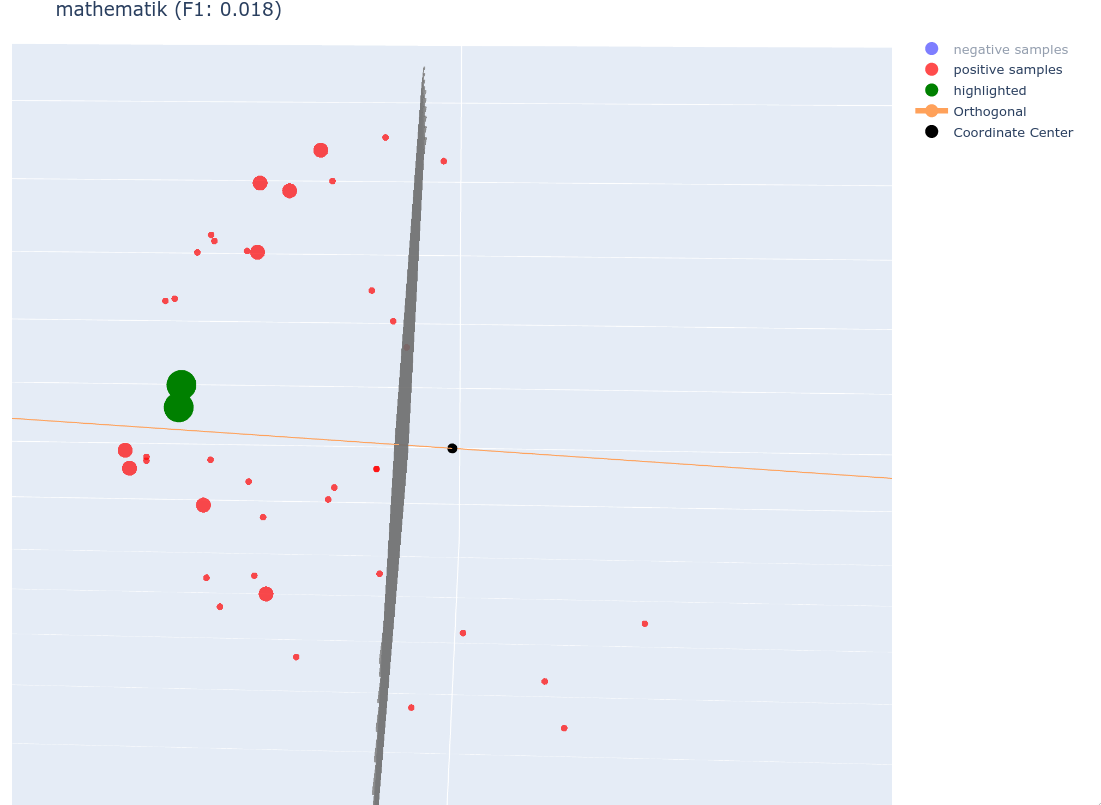
\includegraphics[width=\figwidth]{svm_mathematik_highlight_infoAB.png}
	\caption[3D-Plot with an SVM for the term \textit{mathematik}]{
		\label{fig:3dplot_mathe_infoab}
		3D-Plot with an SVM for the term \textit{mathematik}, also highlighting the courses \textit{Informatik A} and \textit{Informatik B}. Negative samples are hidden for better visibility, and entities that contain the word more often than the 75\textsuperscript{th} percentile have bigger markers.
	}
\end{figure}

\autoref{fig:3dplot_mathe_infoab} displays a 3D-Embedding for courses, splitting courses which contain the term "\textit{mathematik}" from those that do not, also hightlighting the courses \textit{Informatik A} and \textit{Informatik B}. Both courses are close to each other for both the \textit{normalized angular distance} and also euclidean distance.\footnote{Normalized Angular Distance: Average 1.00, Info A and Info B: 0.37 (Percentile 8.2), Euclidean Distance: Average 0.88, Info A and Info B: 0.39 (Percentile: 8.9)}
Further, even though neither course description contains the word \textit{mathematik}, both courses would receive high values for this feature, indicated by the distance to the decision plane.\footnote{Both statements are better visible in the interactive version of the plot}

% * Seems to be the case, also nice that they are on the mathy side
% * Also holds for other stuff like language ourses, mathe für anwender 1 und 2, etc.

% \subsubsection*{Robustness}

% bei mir halt einfach für die verschiedenen configs laufen lassen, die resulting direction clustern und counten wie viele verschiedene terms vorkommen (gehirn vs psyhologie), ob einige besonders oft rauskommen und wi nah (cosine) die sind -> ROBUSTNESS ASSESEN

% How many unique in sum are there (out of 53 possible)

% Mathematik/Informatik: 22,
% Wirtschaftswissenschaften: 34,
% Rechtswissenschaften: 18,
% Sprach-/Literaturwissenschaften: 23,
% Humanwissenschaften: 23,
% Biologie/Chemie: 35,
% Physik: 37,
% Kultur-/Geowissenschaften: 21,
% Erziehungs-/Kulturwissenschaften: 29,
% Sozialwissenschaften: 29


% \autoref{tab:highest_ranking}

\subsubsection*{Are top ranking courses for the directions convincing?}

To further analyse the quality of the results, we are interested in the top courses of those directions that best represent the different faculties. \autoref{tab:highest_ranking} displays the most prototypical examples for each of those, which is directly derived from the rankings induced by the classifier.

\begin{table}[H]
	\makebox[\textwidth][c]{
	\resizebox{1.1\textwidth}{!}{%
	\begin{tabular}{@{}rcl@{}}
	\textbf{Faculty} & \textbf{Top Direction} & \textbf{Top Course for Direction} \\
	\midrule
	\textbf{Erziehungs-/Kulturw.} & \specialcell[c]{erziehungs-\\wissenschaft} & BA GM 3.2: Der Kinder Zukunft aus elementarpädagogischer Sicht \\
	\textbf{Rechtswissenschaften} & schuldrecht & Strafprozessuales Ermittlungsverfahren, [...] \\
	\textbf{Wirtschaftsw.} & fallstudie & WIWI-B-18001-WI: Management Support Systems B I (BI-Praktikum SAP/BW) \\
	\textbf{Kultur-/Geow.} & stadtgeographie & Mittelseminar/Angewandtes Seminar: Geographische Handelsforschung [...] \\
	\textbf{Mathem./Informatik} & mechanik & Technische Mechanik IV für Maschinenbau \\
	\textbf{Sprach-/Literaturw.} & \specialcell[c]{deutschen\\literatur}  & Deutsch - diachron: Historische Linguistik und Sprachwandel in der Gegenwart [...] \\
	\textbf{Humanwissenschaften} & gehirn & Willensfreiheit und Hirnforschung [...] \\
	\textbf{Physik} & klar & B1-B2 Schwedisch Erweiterungskurs: Schweden - das Land und die Menschen (DIGITAL) \\
	\textbf{Biologie/Chemie} & stattgefunden & Transformation wohlfahrtsstaatlicher Regime in Europa: Aktuelle Forschungskontroversen \\
	\textbf{Sozialwissenschaften} & parteien & Modul Vergleichende Politikwissenschaft I: Westliche Regierungssysteme im Vergleich \\
	\end{tabular}
	\caption{Highest ranking courses per feature that best predicts the faculty}
	\label{tab:highest_ranking}
	}}
\end{table}

Again we observe that many of these make intuitive sense, but \textit{Physik} and \textit{Bio/Chemie} cannot be satisfactorily captured by our dimensions. \textit{Mechanik} was an unfortunate choice to encode \textit{Mathematik/Informatik}, however the corresponding course for the \textit{direction} definitely seems resonable.


% \paragraph{concluding remarks}

% In general we must say that we have really good accuracies and this really seems to indicate that it works.  We could to the shallow-decisiontrees-thingy for other attributes of the dataset than we currently have (see future work)

\subsection{Hyperparameters results}

After much preliminary elimination of other techniques, we decided on 165 different hyperparameter-combinations for the final run, which are what was decided on in after much preliminary elimination of other techniques.\footnote{An exception to this are of course the results for three dimensional spaces, which are not competitive and only generated because they are more intuitive and presentable.} For example, prior experiments have shown that the \textit{reclassify} algorithm to find cluster directions outperforms the one used in \cite{Derrac2015}, which is why the latter was not considered in the final evaluation, to counteract a combinatorical explosion of hyperparameters.\footnote{With regards to this specific parameter, there is however qualitativ evidence given in \autoref{tab:text_per_dim}.}

\paragraph{Classifier-Scoring-Methods}

Let us first consider if the choice of the exact evaluation method to quantify the classifier performance is relevant. For that, we look which score leads to the best result, and if the results differ drastically. \autoref{tab:kappa_table} clearly indicates that the algorithm is very susceptible for the exact scoring method used. It was to be expected that comparing raw counts to rankings performs worst (column \textit{c2r+}), and that was confirmed. Besides this, it is also interesting how big the difference between \textit{rtr2+min} and \textit{r2r+max} is, considering that they only differ in how they deal with duplicates. It was suprising that \textit{digitizing} the values 
worked at all. We see that the only scoring-methods that produced enough (2*\#Dims) cluster-centers are those that only considered those terms that occur at least once, which makes sense given that otherwise the scoring was too much influenced by the number of elements in the positive class. 

To get a better grip on the algorithm's robustness with respect to the exact scorer choice, let us now also consider their overlap as printed in \autoref{tab:kappa_overlap}. %\todoparagraph{Was waren die anderen hyperparams fur diesen run???}

Some things we see include:
% \todoparagraph{Yo chris diese interpreationen kommen von ner alten version der tabelle ups !! NOCHMAL ANGUCKEN!!}
\begin{itemize}
    \item binary kappa and F1-score have a high overlap (kappa being a bit stricter)
    \item comparing rankings of only the positive values and their digitized versions leads to the exact same results
    \item all of r2r+min/dig+2, kc2r+ are in b2b
    \item all of the onlypos-statistics are completely in the respective kappa bin2bin
\end{itemize}

Furthermore, looking at the individual scoring methods also provides insight with regards to the question if the different nature of our dataset needs to be accounted for: As established, a very important difference is that more relevant words do not occur more often in the Siddata-dataset. This makes it a reasonable assumption that scorers that evaluate the \textit{rankings} should perform worse: If it is not the case that important words that are very relevant to an entity necessarily occur more often in its associated text, comparing its ranking should perform worse than considering the classification as a binary problem. 

We can test that by comparing the overlap of features that achieve high kappa-scores with those that achive high scores of binary metric such as \textit{accuracy, precision, recall} and \textit{F1}. \autoref{tab:kappa_overlap} indicates first that the binary metrics are a lot less strict than the kappa-scores: All those terms which exceeded the threshold of 0.5 for one of the kappa-scores also did so for accuracy and recall. For \textit{precision} and \textit{F1}, however, this is not the case. More evidence is that the kappascores are a lot worse on count than they are on \glspl{quant}. Furthermore, the kappascores are a tiny bit better on lemmatization than without it, providing even more evidence, as it is to be expected that this configuration has a slighly higher word count.
 
\paragraph{Other Hyperparameters}

Note that the results reported in \autoref{tab:kappa_table} were considered \wrt deciding which ones to take for the final runs. This refers only to the decision which scoring methods to use but also about the hyperparameters up to that point - if not at least 2*ndim candidates for clustercenters are generated, the config is useless. In fact, it can be assumed that more extracted values are generally better, because if only the minimal number is generated all of them will become cluster center no matter their degree of collinearity, which makes the resulting space useless. With that in mind, \autoref{tab:kappa_table} suggests that a parameter-config with 200 dimensions that \textit{tf-idf} will tend to produce most dissimilar candidate directions.

In general, the results for different hyperparameters in terms of classifier performance (\autoref{tab:best_params}) indicate some trends:

For one, it definitey shows that comparing the raw count with these rankings performs worst, indicating that while the wording in \gencite{Derrac2015} was ambiguous, they likely talked about comparing the respective ranks. The second predictor of below-average scores is the usage of a three-dimensional embedding. This was to be expected, and given the low expressive power exptected from a three-dimensional embedding, the observed scores are even surprisingly high.

Comparing PPMI and tf-idf as scoring methods does not show any clear trends, however we can also not find good reasons to prefer the former over the latter. Given that calculation of PPMI-scores relies on huge matrix multiplications which are computationally inefficient, we would suggest to use the well-known well-optimized tf-idf score instead. Another insteresting observation is that scoring the Candidate-Matrix differently than frequency matrix of the texts is competitive with using equal scorings for both. Also, even using the raw count for the candidate-matrix did not perform very badly, serving as our final piece of evidence to see the robustness of the algorithm for datasets like ours.

Besides these observations, the other hyperparameters did not seem to affect classification performances much. In the printed table, the highest score is yielded by a 200-dimensional embedding with tf-idf encoding. However the results slightly varied for different random seeds due to differing elements ending up in the train- and test-set, leading to slightly different results with another hyperparameter-configuration ending up slighly better than the one printed in this thesis.

% * interstingly, even with ony 3 dimensions we extract hundreds of params (wtf - doesn't the later table say 3d always sucks?)


% Im allgemeinen muss man sagen die waren nicht so wichtig. When , what config we received was really mixed, sometimes 50d was best, sometimes 200d. 

% * The calculation How to find the best threshold for candidates
%     * did the threshold help?

% \todoparagraph{As exptected, 3D is not too good, and we see that the best combination is blablabla}

% \todoparagraph{What do we see? We see that tfidf is besser than ppmi blablabla}


% \includeMD{pandoc_generated_latex/5_hyperparamresults}


% So what else do we see in the hyperparams?
% * obviously 3d is worst, often didn't even have 6 values with kappa > 0.5
% * Did lemmatizing help?
% * was ppmi better than tf-idf? on par? worse?
% * was the 80 words threshold good?
% * were we correct in assuming that accuracy may be better than kappas? (no)

% TODO: generally write about if Kappa is a good choice (see eg \url{https://en.wikipedia.org/wiki/Cohen%27s_kappa})


% \subsubsection{Our algorithm improvements}

% our reclassify is better tan the desc15-algo (\ref{tab:text_per_dim}).

% \todoparagraph{The different find-name-was??}

% we wrote before that "taking all words as candidate and running a \gls{pos}-tagger led to suboptimal results in previous experiments, which indicated that the robustness of the algorithm is increased if less candidates are used. This will be forther elaborated in the discussion." -> say something about the number of candidates and how its better the way we do it.



% \subsubsection{Robustness}

% first is nsamples, second is maximal number, last is max number
% For 50D:  38 3800 1003
% For 200D: 15 6000 1707


% Robust meaning here that multiple runs yield similar results. We said before that in word2vec the actual directions of the vectors are completely incomprehensibly dependent on the random initial conditions, and we also said that that is an absolute no-go in conceptual spaces.

% Already here go into detail how unrobust the implementation of derrac and the others is. 

% Show and interpret results for how robust my implementation is and if close words are close

% ..then again elaborate that explicit word choices are not too relevant and also not tested here and that we already experimented with different techniques (see appendix for keybert vs the others) but that there is no formal way to test them.

% We hypothesize (see \autoref{sec:extract_cands}) that the reason we are having more robust results than \cite{Derrac2015} is among others because we have less candidates.

% Results of multiple runs: 

% from all the 165 different param-kombis we did, the following had enough (ndims*2) kappas-over-0.5:
% \{3: 40, 50: 38, 200: 15\}

% \subsubsection*{Stuff that we could have done}

% Are the phrases making up the semantic-direction-clusters similar?
% Are there dimensions encoding the COVID-19 pandemic?
% Is there a direction capturing advanced courses?
% Nen Plot der closeness im embedding mit levensthein-distanz und anzahl-gleicher-wörter korreliert und schaut wie explainable das ist

\subsection{Did we achieve the thesis goal?}

Let us now take a step back and answer the question if the results indicate that we achieved the aims of this work. For one, there is certainly more work to do to increase robustness of the results in the sense that an unambiguous name for the resulting semantic direction comes up without being affected much by precise hyperparameter choices or random seeds. The fact that we have tested only by comparing how good the classification can be predicted is also a drawback, but a human study would be clearly outside the scope of this work.

Our results and analysis reach all expectations set in \autoref{sec:success_conds}: We have extensively analysed the difference between the Siddata-dataset and the originally used dataset. Though many differences between the datasets have been found, it has been shown that the algorithm can make sense of the dataset regardless. All results printed in this work are open-source and the original notebooks are freely available to prove that we did not cherry-pick any results for the analysis performed of the previous section. The semantic directions we have found allow to predict a courses' faculty, which encodes an important feature for the recommendation of educational resources. Our performances to predict the faculty even outperforms a classification relying on \gls{bert}.

% \includeMD{pandoc_generated_latex/5_2_siddata}

\section{General Algorithm}

% Now that we seen the algorithm in action and painstaking implemented it we are experts on the algorithm of \textcite{Derrac2015}, so let us critically reflect on the algorithm as such.

After having presented and meticulously implemented the algorithm of \textcite{Derrac2015}, we are familiar enough with the relevant theory and practice, allowing us to now critically reflect on the algorithm in general.

\subsection{Algorithm idea}

When first looking the algorithm of \textcite{Derrac2015}, it appears astonishingly specific. However after having read Gärdenfors' book \textcite{Gardenfors2000a}, the idea for their algorithm is self-evident: In it, Gärdenfors suggests that conceptual spaces can be generated from high-dimensional sensory input by using \gls{mds} to project the original data into a Euclidean space to do geometric reasoning in that space. The book has an entire chapter on computational aspects, in which the author discusses vector space models, dimensionality reduction techniques an \gls{ann} architectures for different levels of human conceptualization. According to that, MDS is especially good at dealing with pairwise distances judgements from a subject's perception, to create a more \textit{economic} representation for \textit{phenonemal} \glspl{cs} \cite[221]{Gardenfors2000a}. \textcite{Derrac2015} did not create the space from sensory data but from text corpora, where the distance of two texts can be measured by the words they share. Their algorithm reasonably combines the idea to generate \glspl{cs} with the steps for a classical \gls{nlp} pipeline as described by \cite{Turney2010} (\autoref{sec:vsm_construction}) Given that, the core contribution of \cite{Derrac2015} mainly lies in the idea that the \textit{faithfulness} of a potential direction for the resulting semantic space can be assessed by the performance of the corresponding decision problem.

\paragraph{Measuring the Faithfulness of directions}

It seems reasonable that this assumption holds for the datasets originally considered by \textcite{Derrac2015}. As extensively discussed, when concatenating reviews of movies or tags describing pictures of places it is natural that words that describe a salient feature of the respective entity occur more often. The Siddata-dataset consists of short descriptions without this property, where most words have a relative document-freqeuncy of less than a percent. However, the technique of comparing the ranking induced by the classification with the score of the words still yielded enough results, and the directions seem to consist of interpretable properties. This surprisingly confirmed the robustness of the algorithm in that regard.

% Under the assumption of the \gls{distribhyp}, the assumption that this is possible seems reasonable. \todoparagraph{Naher drauf eingehen warum? Ich kann nicht einfach distributional hypothesis sagen und fertig}

\subsubsection{Requiring MDS}
\label{sec:discuss_mds}

\textcite{Derrac2015} explicitly state that MDS is the best dimensionality reduction technique for their algorithm, as it is one of the few ones that result in a metric space. In their paper, they describe SVD (the mathematical algorithm behind \gls{lsa}) as a popular technique for dimensionality reduction, but further state that \q{SVD produces a representation in which entities correspond to vectors, which should be compared in terms of cosine similarity rather than Euclidean distance. [...] However, we can expect that spatial relations such as betweenness and parallelism [...] are not meaningful in the representations derived from SVD} \cite[14]{Derrac2015}. These relationships are required for semantic classifiers which mimic analogical and betweeness-based reasoning, which they demonstrate to work for all of their domains. However, this space does not have semantic directions. The \textit{final} feature-based representation of the entities is reached by ranking each entity for each of the feature directions and creating new vectors from these ranks. As acknowledged by \textcite[22]{Derrac2015}, the feature vectors are not orthogonal, not linearly independent and only of ordinal scale level, withhout meaningful distances. \textcite{Derrac2015} create semantic classifiers both for the \textit{intermediate} space with meaningful distances (geometric betweeness- or parallelism-based classifiers) as well as for feature-based representation (a-fortiori-classifiers, see \autoref{sec:reasoning}). However, \textcite{Ager2018,Alshaikh2020} are only interested in the latter space and its resulting feature axes. If that is the case however, it becomes irrelevant if the intermediate space is metric or not, which enables for other algorithms to be used in that step. As stated in \autoref{sec:dim_red}, LSA may be the better choice as it explicitly detects latent topics in descriptions instead of relying on words that are explicitly mentioned. This may also lead to other desirable properties such as comparability of documents and phrases.

If for the explainable classifiers the relevant space is the one with semantic directions, geometric properties of the intermediate space are irrelevant. Instead one should try to generate a space that has both a useful metric \textit{and} interpretable directions. Depending on what the authors consider to be the end result of their algorithm, only one of these necessary requirements for conceptual spaces is fulfilled. So if their end-result is the intermediate space, that is nothing more than a normal \gls{vsm} with some interesting but long-term useless geometric properties. Instead, another possibility may be to calculating a new orthonormal basis on the coordinate system. The next step would then be to enforce orthogonality of the semantic directions as good as possible, and using linear algebra for a change of basis for the entites, such that not only their ranks but their exact position for each semantic direction (axis) is relevant. Subsequently, one could use techniques like Principal Component Analysis to decorrelate the directions. In this way, one would obtain vector without a name, which however could again be found with techniques that rely on \glspl{cos} such as LSA.

\textcite{Ager2018,Alshaikh2020} both do not this interim space and only use re-embedded one, but retain the use of MDS regardless. To our best understanding, they have no reason to do so, giving impression that they read to use MDS in Gärdenfors' book and then forgot that their final re-embedding step makes that irrelevant. 

\paragraph{Using classical techniques}

In fairness, \cite{Ager2018,Alshaikh2020} both experiment with modern neural embeddings for the entities such as averaged \gls{word2vec} or \gls{doc2vec}. Both authors report that this decreased performance (see \autoref{tab:f1_placetypes_long}) compared to their MDS-condition.\footnote{Even though \textcite{Alshaikh2020} state in their paper that relying on better embeddings such as \gls{bert} \cite{Devlin2019} may lead to better results.} However, while they use neural embeddings, they do not adjust any of the later steps to regard for that: they just replaced the \gls{vsm} generated classically in the first steps of the algorithm with a neural embedding, such as averaged GloVe embeddings \cite{pennington2014glove} of the words in the text. On that they ran the exact original algorithm of creating a frequency matrix from the \gls{bow} and using a linear classifier to get the direction. 

% \todoparagraph{Wenn man schon embeddings nutzt dann soll man auch die eigenschaft dass die sinnvolle richtungen haben nutzen. Und wenn man dann shcon mit vektoren arbeitet dann kann man auch lsa undso nutzen. Und dann hat man auch nicht mehr das problem mit too-small-positive-class}

They do not consider looking for latent topics or make use of the algebraic properties that are given for these embeddings (see \autoref{eq:w2vregularity}). A possible avenue could be to look for shared vector components of entity-embeddings and candidate-word-embeddings. Instead, they still rely on the usage of linear classifiers that split according to frequency matrices. We will look more detailed into that soon, but this makes much more sense for \textit{points} in Euclidean spaces than it does for \textit{vector} embeddings where the space is built up from a cosine-distance-similarity-based objectives (see \autoref{sec:mds}). Instead of that, it seems the better idea to take advantage of dealing with vectors, such as the fact that they are inherently directional already. As discussed in \autoref{sec:lsi}, it seems that the concepts of \gls{lsi} to compare the similarity of documents and candidate feature directions seems more appropriate. This has added benefit that not only words literally occuring in the respective texts can be considered, which among others counters the previously stated problem that the used classifiers deal with heavy class imbalance as well accounting for polysemy and synonymy.

% \removeMe{

% \todo 
% \paragraph{Other things}
% Their last step to cluster the good-kappa-ones is very basic and has much room for improvements, see my suggestions.
% Their merge-cnadidate-step (alle nehmen und die zum closestem herclustern und dann die richtung des $T^0.5$ übernehmen) also has much room for improvement, see my suggestion for another algo - we did implement already some stuff but many better ones are imaginable (see future work)
% better ways of getting rid of irrelevant clusters (see my suggestion and also problems with stopwords)

% They do one SVM per term and then cluster similar ones. Ther terms sometimes occur only in like 50/15000 entities, so the validity of the kappa is should be doubted. \cite{VISR12} and many others first try to find latent stuff, which would improve that by a lot because its a lot less sparse. ("contains-one-of-the-terms" is a lot more than "contains-this-term" - that knowledge is also used by the postprocessing of Ager even though shitty.). According to \cite{Derrac2015} there are no methods that keep a metric space, however as discussed for our aim we can drop that.

% \paragraph{Robustness}

% \todoparagraph{We discussed Robustnes before!}
% An algorithm that is so unrobust \wrt its precise parameter-choices seems a bad choice for conceptual spaces in general. A big issue why we disregarded VSMs is because of their arbitrary dimensions!

% }

\subsection{Does the algorithm actually produce a Conceptual Space?}

\autoref{sec:cs} explained what a conceptual space is, before introducing \gencite{Derrac2015} algorithm to automatically induce them. However, their algorithm only approximates \glspl{cs} and does model some parts of the definition. A first difficulty with the algortihm is, that it needs a clearly defined domain from the start. It takes a corpus of texts and embeds each of these into a single high-dimensional vector space. If not all texts in the corpus are from a single domain, due to the similarity-based vector space generation, outliers will greatly affect the embedding of all entities (as \cite{Ager2018} discusses at length). This sounds irrelevant in practice, but the problem is that it is impossible to clearly define what a domain is. There is the set of place types, but this domain consists of various subdomains, and some concepts apply only to a specific subset of entities. The described algorithm cannot figure out such subdomains. This issue is partially addressed by the works of \textcite{Alshaikh2019, Alshaikh2020, Alshaikh2021} which elaborate on the idea of subdomains. As they state, \textit{\q{When representing a particular entity in a conceptual space, we need to specify which domains it belongs to, and for each of these domains we need to provide a corresponding vector.}} \cite{Alshaikh2020}\footnote{Their improvement to the work of \textcite{Derrac2015} is many to introduce the concept of sub-concepts to the algorithm by hierarchically disentangling the generated space into subfeatures that only exist if certain top-level features are given, such as encoding the \textit{political orientation} of Organizations only for those have a high degree of being \textit{political} in general.} 

Also it is important to be aware of the difference between what \mainalgos and this work consider a domain (the set of movies, places or courses), and the definition of domain as used by \textcite{Gardenfors2000a}. According to the latter, a domain is a low-dimensional set of correlated properties, such as \textit{the color domain} consisting of \textit{hue, saturation} and \textit{value}. This also points out another difference of the original \gls{cs} definition and the definition used here: Conceptual spaces describe an entity through several uncorrelated low-dimensional vector spaces, not a single one with several dozen dimensions. As \cite{Ager2018} puts it more humbly, \textit{\q{The idea of learning semantic spaces with accurate feature directions can be seen as a first step towards methods for learning conceptual space representations from data [...]}}. Again it is referred to the works of \textcite{Alshaikh2019, Alshaikh2020, Alshaikh2021} which alleviate this by iteratively finding disentangled low-dimensional feature spaces.

As discussed earlier, the algorithm of \textcite{Derrac2015} first embeds the entities into a Euclidean space where the concepts of betweeness and parallelism make sense, and subsequently create a feature-based representation that bases on an entity's rank \wrt several human-interpretable features. The final embedding is only of ordinal scale level and thus unable to model  degrees of similarities. In other words, the algorithm produces \textit{either} a space with a euclidean metric, \textit{or} one with interpretable directions, but no space that has \textit{both properties}. As both are necessary conditions for a conceptual space, \gencite{Derrac2015} algorithm at no point generates something that resembles a \gls{cs}. It remains unclear to us why they only consider the ranking of the entites regarding the feature axis instead of their distance which may retain relations of distances, for example by applying an arithmatic change of basis for the coordinate system (linear transformation). The way their algorithm works, the final space only has ordinal scale level and linearly dependent (correlated) dimensions. An interesting research avenue is to figure out what properites the space they have, and if small changes to the final algorithm step (such as \gls{pca} to decorrelate dimensions or not only taking the rank) could help in retaining the euclidean or at least another usable metric.

\subsubsection*{Points instead of Regions}

Another important difference between the resulting space and \glspl{cs} is that we are dealing with points instead of regions. Advantages of doing that include that it allows to distinguish \textit{protypical} examples from borderline cases \cite{Gardenfors2000a} and straight-forward application of ontological relations through the \gls{rcc} (see \autoref{sec:ontology_rcc}). \textcite{Derrac2015}, however, drop this assumption and work with vectors instead of regions, claiming that this is a \q{coarse-grained approximations of conceptual spaces, where points correspond to fine-grained categories instead of specific instances, while convex regions are used to model higher-level categories} \cite[8]{Derrac2015}. Despite that, they never address it again, so in the end they stick with points. This breaks with one of the key concepts from \glspl{cs} and also renders it impossible to simulate any of the ontological relations with the resulting spaces, which Gärdenfors considered their most relevant practical application \cite{Gardenfors2004}. 

However, when elaborating on the idea that conceptual spaces can be induced using Kohonen-Nets (\autoref{sec:algo_variants}), Gärdenfors himself claims that mapping regions of the original space to point-embeddings in the \gls{cs} is an \textit{advantage}, because it resembles \textit{generalization}. Another aspect to consider is whether the \glspl{entity} as considered by \mainalgos actually resemble what Gärdenfors originally considered an entity. The entities in the used datasets of educational resources, placetypes or movies actually are specific instances instead of general \textit{concepts}. Instances in a conceptual space are correctly modelled as points - one could say that regions denote \textit{types}, with the individual points corresponding to their \textit{tokens}. Considering that we have only one instance per entity, we are dealing with types. Concepts (Regions in a CS) could accordingly be induced as the set of multiple tokens. A practical implementation could, for example, model the concept of \textit{introductory computer science courses} as a convex region spanned by all of the instances it contains. \textcite{Erk2009} propose an algorithm that creates such a region with varying variances per dimension from a set of prototypical instances. It should be noted, however, that learning boundaries for such regions requires much more data \cite{Derrac2015} and the aforementioned reasoning on regions is computationally very complex \cite{Hernandez-Conde2017}.


\paragraph{Vectors or Points}
\label{sec:discuss_points}

The authors explicitly claim that they are dealing with points in a Euclidean space, which should be compared in terms of Euclidean distance \cite[14]{Derrac2015} instead of \gls{cos}. Despite this, in the merge-canidates step of their algorithm (\autoref{sec:algo:cluster}), they compare the candidate feature directions using the \gls{cos} of their orthogonals. As they require similarity of directions and not of positions, this approach seems plausible. However, these vectors do not have their origin in the coordinate base but in the position where they cut across the SVM's decision surface: A SVM is described by the vector of its orthogonal intercept, a scalar describing where the decision hyperplane crosses it. This means that one is dealing with \textit{affine frames} (which are described by basis and origin) instead of vector spaces. However, vectors in affine spaces cannot be compared solely by the angle between them\footnote{For better comprehension it is referred a StackOverflow question of \me at \url{https://stackoverflow.com/a/69407977/5122790}}. The way their algorithm is described, their merging of feature direction disregards the origin. Consider the following example: The SVMs for two candidates have exactly the same orthogonal vector, but different intercepts. There might be samples between the two decision surfaces, which are classified towards the positive class by the one classifier, and towards the negative by the other. If they classify samples differently, they must express different concepts. When only accounting for the direction of the orthogonal, such information gets lost. 

\subsection{Outlook}

There are also techniques that extend the algorithm of \textcite{Derrac2015}: \textcite{Alshaikh2019} take a vector space embedding and decompose it to several low-dimensional spaces, such that it corresponds more closely to the definition of a \gls{cs} which are split into multiple domain-specific spaces of low dimension. For that, they take the spaces from \cite{Derrac2015} to then cluster their features by domain and iteratively remove these groups to create multiple subspaces, while ensuring that \gls{word2vec} embeddings close to those of the removed ones are disregarded for future features.

\textcite{Alshaikh2021} want to get rid of MDS with its quadratic space complexity and also write a completely new, unsupervised ANN algorithm based on GloVe embeddings \cite{pennington2014glove}. In it, they learn domain-specific embeddings from the BoW and like \cite{Derrac2015} use classification, splitting entities that contain one of the verbatim candidates vs. those that do not. They train an \gls{ann} on this while also punishing close embeddings, similar to their previous work \cite{Alshaikh2019}.

% \subsection{Regarding their research practices}

% In \autoref{sec:howtoreplicate}, we stated the importance that all claims made in research should be reproducible and testable. While replicating the work of \cite{Derrac2015}some Questionable Research Practices came apparent. For example, 



% \paragraph{Robustness}
% \todo

% \paragraph{Ambiguity}
% \todo




% \includeMD{pandoc_generated_latex/5_3_evalderrac}




\section{Architecture}

As one of the thesis goals asked for a good and scalable architecture, we will also evaluate whether the implementation fulfills the set criteria (\autoref{sec:success_conds}) and if the aspects we considered for a qualitative software and sustainable data analysis (\autoref{sec:reproducibility}) are fulfilled.
% We remember, we also wanted to build a good architecture and set goals for that, such as adaptability to new datasets etc. We said a good architecture would show in adaptability, scability, ..., so we wanna show that these are achieved. 

First of all, we wanted to show that this implementation works and is able to replicate the results of one dataset of \mainalgos. This aim was reached, indicating \textbf{Functional Suitability} of our implementation and also the \textbf{Reproducibility} of the original algorithm.\footnote{If our implementation itself is reproducible can hardly be shown by \me in this thesis.}

Another goal was that the code-base successfully runs on the \gls{ikw} compute grid. This goal was also met, and the resulting implementation and its \textbf{Automation} and \textbf{Scalability} proves satisfactory. Testing new hyperparameters is as easy as changing a YAML-file, transferring the file to the grid and executing a command\footnote{such as \codeother{MA_ENV_FILE=siddata.env submit by_config --configfile config/CONFIGFILE.yml}}. The maximum number of cores per node and of nodes available to a user (64) are maximally utilized, which also indicates optimal dependency resolution. Running the algorithm on sample datasets worked without any complications in a matter of minutes (\textbf{Modularity, Maintainability, Adaptability}).

Allowing for all this was surprisingly intricate. Having worked with \textit{Snakemake} on clusters before, the amount of customization to allow for workflow management on the \gls{ikw} grid was surprisingly high. This was partially due to heavy iterative restructuring of the code-base to comply with the logic as demanded by this workflow management system. Part of this is due to peculiarities of its configuration,\footnote{For example that \textit{accounting files} that keep track of jobs are inaccessible to users, which means that our scheduler needs to simulate their behaviour.} but also to a huge degree due to the walltime-limit of 90 minutes. Because of this, most of the algorithm components need to be written in a way such that they both massiveley parallelize, but also gracefully end and store interim results, and the scheduler must comply with this. Comparing this with the uploaded implementation of \cite{Alshaikh2020}\footnote{\url{https://github.com/rana-alshaikh/Hierarchical_Linear_Disentanglement}}, which consists of one Jupyter Notebook and one Python file, gives indication of the amount of work necessary to reach this. We sincereley hope that this thesis helps in \textbf{Transparency} and that at least the cluster execution will be re-used by other students of the \gls{ikw}.

All the analyses that were conducted for this thesis are given in the accompaning source code. All plots and tables from all previous sections that were not reprinted were created in publicly available Jupyter-Notebooks, together with many more analyses that were conducted but would go far beyond the scope of this thesis. All plots and tables are explicitly linked and easily re-creatable and runnable. A lot of work was put into the architecture, and as soon as architechture and worklow management worked as intended, further development on the algorithm was suprisingly quick. This indicates that the general aim of creating an architecture that helps to answer related future research questions is fulfilled. For the sake of brevity, this analysis and the code-base itself, which is available at \url{https://github.com/cstenkamp/derive_conceptualspaces} shall suffice as explanation regarding the final two set goals. 

% \removeMe{
%     \todoparagraph{IN 3_3_architecture is a section} "My workflow to generate results", darauf nochmal eingehen und sagen dass das wirklich wunderbar funktioniert, dass es am ende nur ein wenig chaotisch ist weil man darauf achten muss dass man consistent ist in den conditions für best-config (random seed für die decision trees undso)
% }


% \includeMD{pandoc_generated_latex/5_4_architecture}

\section{Future Work}
\label{sec:futurework}

While this work has shown that the general technique seems to work, so far it has not produced an actual recommender for edcucational resources. Accordingly, building an interface as \eg the one from \autoref{fig:movietuner}, or alternatively a textual interface that relies on a dialogue with a user to generate recommendations is an important direction for future work. When this is added to the Siddata-\gls{dsa}, this may directly be combined with a study in which the users volunteer information about the usefulness of recommendation or even providing possible labels, which may be used for algorithm evalution with labels other then the faculty, or even supervised training as done \eg by \cite{VISR12}. Also, more analyses can be performed on the current data, such as correlating distances in the semantic space with \textit{Levensthein-distances} in textual descriptions, or looking \textit{in what direction} individual faculties differ.

\subsection*{Algorithm Addendums}  As stated many times by now, the algorithm that was replicated in this work is very modular and requires only certain types of algorithm for many of its components. While recreating the works of \mainalgos, many smaller and larger changes to the algorithm could have been performed. A complete list of considered algorithm-extensions can be found in this repository\footnote{\url{https://github.com/cstenkamp/MastersThesisText/blob/master/pandoc_markdown_base/futurework_long.md}}. Among others, not all extensions from \cite{Ager2018, Alshaikh2020} have been implemented yet. It may also be insteresting to consider new distance-measures for the entities such as variations of the \textit{Levensthein-distance} or the \textit{Jaccard-distance} (\eg \gls{iou}, as done in \cite{Schockaert2011}). Also, more work is needed to remove irrelevant dimensions, in the hope of making the algorithm more robust. Especially the clustering and merging of similar features may benefit from considering other techniques. These include using \gls{iou} similar to \cite{Alshaikh2019} as similarity measure, methods to remove uninformative clusters, or considering other algorithms for clustering and calculating the centroid directions that weight or threshold based on classifier performance or similarity. Finally, finding a representative cluster name may benefit in robustness from also considering pseudo-documents \cite{VISR12} or other methods, \eg those suggested by \textcite{Carmel2009}.

\subsection*{Complex Changes} Besides the aforementioned additions, there are also many avenues that change more of the algorithm's logic. These include the fine-tuning step of \textcite{Ager2018}, which may be combined with latent topic detection techniques to alleviate the fact that the desriptions of the Siddata-dataset are short and omit many words that may serve to describe an entity. Many other ways to find latent topics may also be considered, such as relying on semantic databases and counting \textit{hyponyms} of candidate directions towards their count for a description, or again relying on vector similarity as demonstrated in \gls{lsa} and also neural embeddings such as \gls{word2vec} and \gls{doc2vec}. We have established that the current form of the algorithm only yields either a space with a Euclidean metric or one with semantic directions. Finding ways to get both would be an important contribution - it is \eg unclear why so far only rankings have been considered instead of linear algebra to find a new coordinate base. Alternatively, one can ignore the requirement of the Euclidean metric completely, which opens up many major changes to the algorithm such as not relying on \gls{bow}-representations at all, but instead using modern document embeddings such as \gls{bert}, where candidates are detected using the \gls{cos}.

\subsection*{New Algorithm}

Finally, let us try to combine all the issues raised in this work to form a suggestion of how a completely different algorithm may look.
First, we want an embedding that retains as much of the original dataset variability as possible. For that, additionally to a small set of absolutely most important dimensions found as the orthogonal of the linear classifiers, one may consider subsequently running \gls{pca}\footnote{PCA is a technique used for dimensionality reduction that works by projecting high-dimensional data onto its \textit{Principal Components}, those directions that explain most of its variance.} to find \textit{remaining} variance for those dimensions that do not obviously correspond to the occurance of single words. This has the additional benefit of finding \textit{orthogonal} directions which helps to get low-dimensional spaces, expressed by a small amount of uncorrelated features. So far, the directions found by \gls{pca} do not have a name, but we have also examined ways such as LSA that find words by their similarity of angles. In fact, it may be possible to build the whole algorithm on the basis of \gls{pca}: Instead of relying on \gls{bow}-representations, texts could be embedded using \eg \gls{bert}, which also takes into account its hidden topics and word ordering. Subsequently, one may run PCA to find a few directions of this space that best explain the dataset variance. Embracing the fact that one is dealing with vectors, \gls{lsa} can then be used to find candidate dimension names which do not rely on exact phrasing of the corpus. A disadvantage of such an algorithm is, that the resulting space is not metric\footnote{Though one may try to use pairwise distances for each of the dimensions to create a new metric space using a variation of MDS, or rely on Kohonen-Networks for that, as suggested by Gärdenfors \cite{Gardenfors2000a}.} - but neither is the space yielded by the algorithm explored in this thesis.



% \includeMD{pandoc_generated_latex/5_0_futurework}

\section{Conclusion}

This thesis explored how explainable generation of educational resources can be generated in a data-driven manner from a corpus of their descriptions. It has been established that \textit{Conceptual Spaces} can serve as knowledge representation method for that by capturing dataset properties in a way that allows to computationally model explainable reasoning. To generate these automatically, the method by \cite{Derrac2015} was thoroughly examined in theory and in practice.

The introduced algorithm was successfully replicated and the results on the originally used data have been confirmed. We have sucessfully transferred the algorithm to the domain of educational resources and demonstrated its ability to find relevant human concepts in our dataset. By means of this, we have demonstrated the robustness of the methodology by discussing the difference in the datasets as well as the respective results. Some adjustments to the original algorithm have been shown to further increase its performance. Analysis on the results of our dataset has shown that surrogate metrics indicate that the algorithm finds some regularities in the dataset, such as a courses' faculty. Despite this, more work to thoroughly test the algorithm's capabilities, but also to increase its performance and robustness will be needed.

To make the replication and application of the algorithm possible, we have implemented a tool that allows to easily recreate the results of \mainalgos. This tool was built while ensuring to comply with code quality standards and proper methodology, is open-sourced and can easily be installed as a package. The result of this is a reliable pipeline that has been demonstated to be easily adaptapted and extended. We hope this helps raising the attention of a broader community to the methodology and enables future research on further varition or domain transfers to be simple, quick and accessible. Another major contribution of this thesis are the solutions that were found to run workflows similar to the one required here on compute clusters, specifically the \gls{ikw} grid. The result is a workflow that is much more versatile and user-friendly than the ones we know to be used to date,\footnote{So far, the only methods that we have seen suggested are to write custom shell-scripts, see \eg the discussion and links in its respect Stud.IP group at \url{https://studip.uni-osnabrueck.de/plugins.php/coreforum/index?cid=e946790f6a74e17df02a85847b2110ab} \acc{04}{09}} and we hope that it helps to make high performance computing more attractive to other \gls{uos} students. All analyses conducted in this work are open-sourced as well and can be easily inspected and re-created.

Finally, we have discussed Conceptal Spaces and \gencite{Derrac2015} algorithm extensively on the basis of our results. We have reached the conclusion that while the algorithm produces reasonable results automatically and shows much potential, it drops necessary assumptions of Conceptual Spaces by not producing a single embedding that is both metric and also has interpretable dimensions. We have concluded that because of this, some assumptions about necessary design decisions can be dropped, which may allow to combine the methodology with state-of-the-art algorithms.

% * Wir haben diskutiert ob der algo sinn macht etc
% * Regaring CS: seems cool. Both in terms of  model of human concept formation AND algorithm-that-allows-certain-things-like-reasoning
% * Regarding the algorithm
%     * That motivated us in the first place: automatically create structured knowledge bases bc explainability. Need is there.
%     * I think it has potential
%         * Is it practical? enough so.
%         * though technically it doesn't create a CS - would be better if we can get both metric and interpretable direcitons. 
%     * I think better algorithms could exist, one should consider using neural embeddings.


% \includeMD{pandoc_generated_latex/5_6_conclusion}